\section{The Critical Path Method}
%Eigentliche Beschreibung der Methode (5 Seiten) - Mathias
% overview:
%http://hspm.sph.sc.edu/COURSES/J716/CPM/CPM.html

The \cpm{} (or just CPM) was originally introduced by James Kelley and Morgan Walker in
\cite{Kelley:1959:CPS:1460299.1460318}. The foundation of the \cpm{} is an abstract notion of a
\emph{project}. A project is assumed to consist of \emph{jobs} that represent individual activities
and are executed seperately from each other. Each job may depend on the completion of other jobs and
in turn must be completed for other jobs to begin. The central goal of the \cpm{} is to compute a list
of \emph{critical jobs}, where a delay in the completion of a job delays the entire project.

The \cpm{} seperates planning from scheduling. In the planning phase, a planner defines all
activities and the order in which they must take place. The planner must also consider required 
technology, resources, people, etc. involved. A scheduler can then use the defined activities to
devise a schedule based on the plan and on costs\cite[p. 161]{Kelley:1959:CPS:1460299.1460318}.

\cpm{} has evolved since its original incarnation to include other aspects essential to the
successfull completion of a project, such as required resources and resource-leveling. Various tools
and techniques have been developed to optimize and shorten the critical path.

\subsection{What you can achieve using the \cpm}
The seperation of planning and scheduling allows the project management to dynamically reschedule
parts of the project during its execution if real-world events force a deviation from the plan.
Reasons for deviation may be a natural disaster, a delay in the shipment of required resources or
a late completion of a critical job. Practical experience shows, however, that rescheduling is a
complex and error-prone task. Moving a job may be simple in theory, but might in fact be very
complex. For example, moving a job to next week might mean that a required specialist is not
available for a different job that is scheduled during that time period.
%TODO: Da gibts ne quelle irgendwo dafuer.

\subsection{Initial planning}\label{subsec:initial_planning}
The first thing when applying the \cpm{} is to draw up a list of activities. This has to take place
\emph{before} any real work is done on the project and might be considered an initial kick-off of
the project. This list can be done in the
form of a \emph{work-breakdown structure} or in any more or less formal structure. The planning team
has to take great care that this stage is done correctly, as any errors could cause big problems
during the execution of the plan.

When the planning team decides on an activity, some information on it should be compiled:
\begin{enumerate}
  \item A unique name. The name should be somewhat descriptive of the activity.
  \item An estimated total time that the activity will take to complete. Depending on the
    requirements, other estimates (minimum time, maximum time, \ldots) might also be of interest.
  \item Activities that must be completed before this respective activity. It is also good practice
    to (informally, at first) write down other activities that depend on the activity.
\end{enumerate}

One important question that should be considered is the level of abstraction the plan should have.
For example, when trying to build a large oil-tanker, it doesn't really make sense to have the
activities "build outer hull" and "tighten screws of the captains chair" on the same plan. The
chosen abstraction of the plan depends on
\begin{itemize}
  \item Who creates the list of activities. The list of activities might even be drawn up by higher
    levels of management and only then handed down to different devisions of the planning
    departement. As such, the activities might already indicate a certain division of work. 
  \item Who will read and work with the plan. A plan based on the \cpm{} might also be used to 
    formally communicate i.e. between different management divisions, autonomous sections of a 
    company or other companies alltogether. Depending on the recipient of the plan and his
    experience and knowledge, the a different level of detail might become necessary.
  \item The overall complexity of the project. For a very large and complex project comprised of
    many different individual activites, a lower level of abstraction might not be practical. A
    possible solution is to logically split the project into individual parts, so that each part
    becomes seperated (albeit depending on each other) from each other. 
  \item Dependency on other activities. A defining axiom of the \cpm{} is that each activity can
    only start when all activities it depends on are fully completed\cite[p. 37]{obrien}. Following
    this axiom, it might become necessary to split an activity A into two parts, if activity B
    depends on the first part of A and the second part of A depends on activity B.
\end{itemize}

One common mistake made in the implementation of the \cpm{} is to assume that software support tools
(see section~\ref{sec:inthefield}) either draw up a list of activities for you or make drawing up
such a list a lot easier. Software support tools do not (and cannot) aim to ease this task, they can
only process the information they receive. If this initial work is not done carefully, any diagrams
etc. drawn by software are not any better than if no software were involved\cite[p. 39]{obrien}.

\subsection{Drawing the activity diagram}
An \emph{activity diagram}, often also called \emph{network diagram}, is the central part of the
\cpm{}. The diagram is created based upon the list of activities devised in
section~\ref{subsec:initial_planning}. 

When an activity is completed, an \emph{event} is said to occur. Such an event has no 
duration but represents an instance in time. Consequently, every activity has a \emph{starting
event} and a \emph{completion event}. Every event has one or more preceding and subsequent
activities, the only exceptions being the starting event (which has no preceeding activity) and the
event that marks the end of the project (which has no subsequent event). Each event is usually
identified by a unique integer.

The most important element of an activity diagram is of course the activity, represented by a simple
arrow. Depending on the complexity of the graph, arrows might be descriptivly labeld or labeld with
references to the actual activity that may be looked up in a reference table. Such a table is needed
in any case to store additional information (such as duration, etc.). By definition, each activity
must be uniquely identifyable by a pair of events $i,j$, denoting the start and completion event.
Figure~\ref{pic:activity_diagram_intro} shows a minimal and abstract activity diagram.
\begin{figure}[h]
\centerline{\fbox{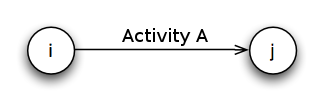
\includegraphics[width=50mm]{img/activity_diagram_intro}}}
\caption{A minimal activity diagram}
\label{pic:activity_diagram_intro}
\end{figure}

Either \emph{dummy events} and/or \emph{logical restraints} may be used in cases where a simple
sequence of activities is not powerful enough to express the dependencies devised during planning. A
logical restraint is an activity that represents no work (and has no duration) and is is drawn as a
dotted arrow. A dummy event is an event added solely for the purpose of expressing dependencies that
would otherwise cause violations of constraints imposed on the activity diagram.

A first use of a dummy event combined with a logical restraint is when two (or more) activities
would normally be identified by the same preceeding and subsequent event. This generally occurs when
two activities have the same set of predecessors and successors.
\begin{figure}[h]
\centerline{\fbox{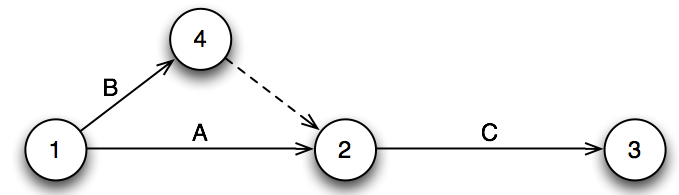
\includegraphics[width=100mm]{img/activity_diagram_one}}}
\caption{activity diagram with dummy event and logical restraint}
\label{pic:activity_diagram_one}
\end{figure}

In figure~\ref{pic:activity_diagram_one}, both activity A and B depend on activity C. Because
activity A and B cannot both be identified by the sequence $1,2$, the dummy event $4$ is added
simply to change the identification of activity B. The dotted line is the logical constraint
defining that activity C depends on the completion of activity B.

\subsection{Adding durations to the activity diagram}
Drawing the activity diagram visualizes logical dependencies between certain activities. This helps
with scheduling activities, but it doesn't yet tell us about which activities are more time-critical
than others. This is of course the information that the \cpm{} is all about: The goal is to find the
\emph{critical path(s)}, one or more sequences of activities that must not be delayed if the project
at hand is to complete in a timely fashion.

The key to this information is to add time estimates of the activities to the diagram. An estimate
might be a "most likely" estimate. Other possibilities are the minimum or maximum amount of time
that an activity might take. More enhanced versions of the \cpm{} may use a combination of different
time estimates, but the original method of detecting critical paths is based on using a single time
estimate. 

A good first start for time estimates is to use the time it might take most likely to complete the
task. If the time estimates are done by a skilled team, additional information might flow into the
estimates. For example, if a skilled team is known to be available for performing the activity, the
estimate might be more optimistic. The estimate might be even more precise if the activity does not
represent a totally new task but some work that was performed in the past already. This basically
means that experience and knowledge of both the planning team and the teams "in the field" should be
considered in any time estimates.

In some instances, it may be very hard to do any correct estimate of the duration of an activity.
This is especially true for activities that have never been performed before. A good approach,
according to \cite[p. 91]{obrien}, is to use a "bracket approach". In this approach, you first take
a very high figure (almost worst case scenario) and a very optimistic figure and try to find a good
compromise between the two extremes.

\begin{comment}
\subsection{Find critical paths}\label{sec:Find_criticial_paths}
The information compiled in the previous sections is now ready to be used to find the \emph{critical
paths} of the project. This is of course the quintessential part of the \cpm{} that gives it a
decisive advantage over a much simpler bar chart or an even simpler todo-list.

Several attributes are calculated from the durations of each activity and the composition of the
diagram. After applying the \cpm{}, each activity has a point in time where the activity may finish
in a best-case scenario. This time is called the \emph{earliest start} or simply $ES$. Each activity
will consequently also have an \emph{earliest finish} or $EF$ for short. The earliest start of the
first activity is by definition the time the project starts, in relative terms simply 0. The
earliest finish of the last activity in the project is also the \emph{earliest finish} of the entire
project. The earliest start of an activity other than the very first activity is the same as the
last earliest finish ($LEF_{pred}$) of all activities that the respective activity depends on. 

The earliest
finish is calculated simply as the earliest start of an activity plus the duration denoted in the
previous section. Because earliest start and earliest finish are by definition calculated from the
start of the project to the end of the project, calculating these attributes is referred to as the
\emph{forward pass} (in contrast to the \emph{backward pass} explained below). The equations in
(\ref{eq:forward_pass}) contain all the relevant formula for the forward pass.

\begin{eqnarray}
&& ES_0=0 \nonumber\\
&& EF=ES+D \nonumber\\
&& ES=LEF_{pred}
\label{eq:forward_pass}
\end{eqnarray}

Using the attributes ($ES$, $EF$) calculated in the forward pass, we can start with the next pass,
the \emph{backward pass}. In this pass, we calculate attributes from project finish to project
start, hence its name. After the backward pass, each activity will have a \emph{latest finish} 
($LF$) attribte, which denotes the time by which an activity \emph{must} be completed. The violation
of a latest finish attribute by definition means that the entire project is delayed. The latest
finish attribute is calculated as the earliest erliest start ($ELS$) of all activities that succeed
it. 

The backward pass also computes the \emph{latest start} ($LS$) of an activity, which simply is the
latest finish minus the duration of the activity. The latestest start expresses the time by which an
activity \emph{must start} if it shouldn't delay the completion of the project. The equation in
(\ref{eq:backward_pass_one}) contain all the relevant formula of the backward pass.

\begin{eqnarray}
&& LF_{end}=EF_{end} \nonumber\\
&& LS=LF-D \nonumber\\
&& LF=ELS_{succ}
\label{eq:backward_pass_one}
\end{eqnarray}

A \emph{second} backward pass enables us to calculate more interesting attributes. The \emph{free
float} ($FF$) is the difference between the earliest start of any succeeding activity and the early
finish of the respective activity. It thus represents the amount of time by which an activity can be
delayed without delaying the entire project.  The \emph{independent float} ($IF$) is defined as the
difference between the earliest early start of any succeeding activity and the latest early finish 
of any preceeding activities. The formulas are given in (\ref{eq:backward_pass_two}).

\begin{eqnarray}
&& FF=EES_{succ}-EF \nonumber\\
&& IF=EES_{succ}-LEF{pred}-D \\
\label{eq:backward_pass_two}
\end{eqnarray}

\end{comment}

%\subsection{Common errors}
%* logical loops
%* express dependencies in diagram that aren't there
%
%\subsection{Possible improvements}
%more information, to shorten project time, assign resources, etc.
%* resource leveling (s. 76 mitte)
